% $Header: /cvsroot/latex-beamer/latex-beamer/examples/beamerexample1.tex,v 1.47 2004/11/04 15:43:51 tantau Exp $

\documentclass{beamer}
%\documentclass{article}
%\usepackage[envcountsect]{beamerarticle}

% Do NOT take this file as a template for your own talks. Use a file
% in the directory solutions instead. They are much better suited.

% Try the class options [notes], [notes=only], [trans], [handout],
% [red], [compress], [draft] and see what happens!

% Copyright 2003 by Till Tantau <tantau@users.sourceforge.net>.
%
% This program can be redistributed and/or modified under the terms
% of the LaTeX Project Public License Distributed from CTAN
% archives in directory macros/latex/base/lppl.txt.

% For a green structure color use:
%\colorlet{structure}{green!50!black}

\usepackage{array,paralist}
\usepackage{tabularx}
\usepackage{eurosym}

\mode<article> % only for the article version
{
  \usepackage{fullpage}
  \usepackage{hyperref}
}


\mode<presentation>
{
  \setbeamertemplate{background canvas}[vertical shading][bottom=red!10,top=blue!10]

  \usetheme{CambridgeUS}
  \usefonttheme[onlysmall]{structurebold}
}

%\setbeamercolor{math text}{fg=green!50!black}
%\setbeamercolor{normal text in math text}{parent=math text}

\usepackage{amsmath,amssymb}
\usepackage[latin1]{inputenc}
\usepackage{colortbl}
\usepackage[english]{babel}

%\usepackage{lmodern}
%\usepackage[T1]{fontenc} 

\usepackage{times}
\setbeamercovered{dynamic}

%% Titel etc
\title[]{Kabellose Sensornetze: ZigBee, Bluetooth \& co.}
\author[Noe]{Marcel Noe}
\institute[TNG]{
        \inst{}TNG Technology Consulting GmbH}
\date[2013]


%% Hauptseite
\begin{document}
\frame{\titlepage}

\section<presentation>*{Einf�hrung}

\begin{frame}
  \frametitle{�berblick}
  \tableofcontents[part=1,hidesubsections]
\end{frame}

\part<presentation>{Vortrag}


\logo{}
\section{Motivation}
\subsection{Was ist ein Sensornetz?}
\begin{frame}
    \frametitle{Was ist ein Sensornetz?}

    \begin{columns}[T]
        \begin{column}{5cm}
            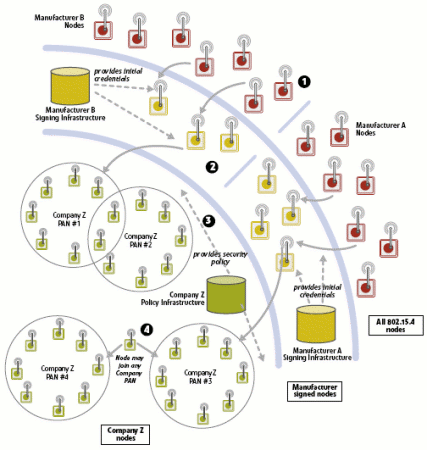
\includegraphics[width=5cm]{images/certicom_sensor_nets_fig2.gif}\\
        \end{column}

        \begin{column}{7cm}
            \begin{itemize}
                \item Foor 
                \item Bar 
                \item Bal 
            \end{itemize}
        \end{column}
    \end{columns}
\end{frame}

\section{Anwendungen}
\subsection{Anwendungen}


\section{Grundlagen der kabellosen Daten�bertragung}
\subsection{Das ISM Band}
\begin{frame}
    \frametitle{Das ISM Band}

        \begin{column}{7cm}
            \begin{itemize}
                \item 6,765 MHz
                \item 13,553 MHz
                \item 26,957 MHz 
                \item 40,66 MHz
                \item 433 MHz
                \item 902 MHz
                \item 2,4 GHz
                \item 5,7 GHz
                \item 24 GHz
                \item 61 GHz
                \item 122 GHz
                \item 244 GHz
            \end{itemize}
        \end{column}
\end{frame}


\subsection{Eigenschaften verschiedener Frequenzb�nder}
\subsubsection{900 MHz}
\begin{frame}
    \frametitle{900 MHz}
\end{frame}

\subsubsection{2.4 GHz}
\begin{frame}
    \frametitle{2.4 GHz Band}
\end{frame}

\subsubsection{5 GHz}
\begin{frame}
    \frametitle{5 GHz}
\end{frame}


\subsection{Frequenzspreizung}
\subsubsection{Prinzip}
\begin{frame}
    \frametitle{Prinzip der Frequenzspreizung}

    \begin{columns}[T]
        \begin{column}{5cm}
            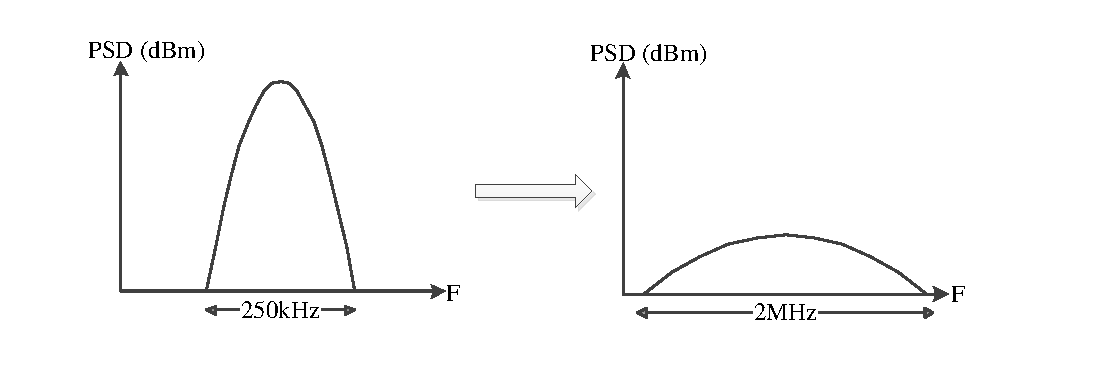
\includegraphics[width=5cm]{images/diplomarbeit/frequenzspreizung_dss.pdf}\\
        \end{column}
    \end{columns}
\end{frame}

\subsubsection{FHSS: Frequency Hopping Spread Spectrum}
\begin{frame}
    \frametitle{FHSS: Frequency Hopping Spread Spectrum}

    \begin{columns}[T]
        \begin{column}{5cm}
            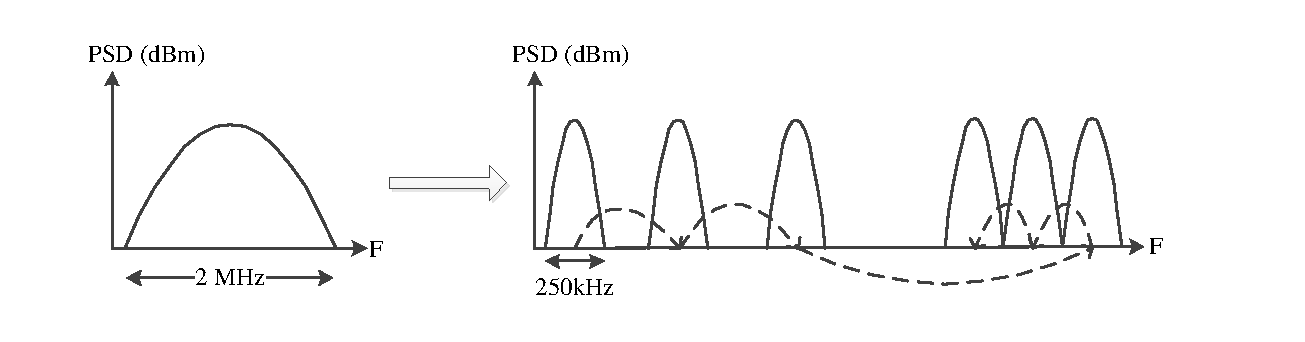
\includegraphics[width=5cm]{images/diplomarbeit/frequenzspreizung_fhss.pdf}\\
        \end{column}

        \begin{column}{7cm}
            \begin{itemize}
                \item Foor 
                \item Bar 
                \item Bal 
            \end{itemize}
        \end{column}
    \end{columns}
\end{frame}

\subsubsection{DSSS: Direct Sequence Spread Spectrum}
\begin{frame}
    \frametitle{FHSS: Frequency Hopping Spread Spectrum}

    \begin{columns}[T]
        \begin{column}{5cm}
            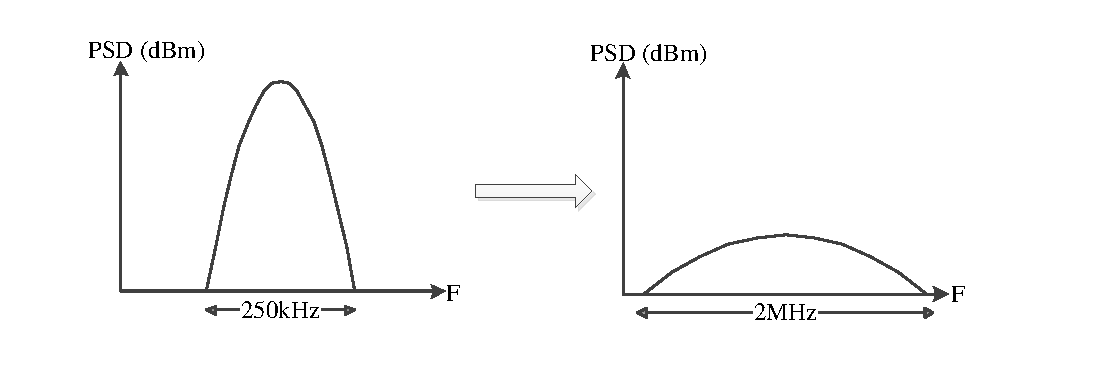
\includegraphics[width=5cm]{images/diplomarbeit/frequenzspreizung_dss.pdf}\\
        \end{column}

        \begin{column}{7cm}
            \begin{itemize}
                \item Foor 
                \item Bar 
                \item Bal 
            \end{itemize}
        \end{column}
    \end{columns}
\end{frame}

\section{Verschiedene Technologien}
\subsection{WLAN}
\begin{frame}
    \frametitle{IEEE 802.11: WLAN}

    \begin{columns}[T]
        \begin{column}{5cm}
            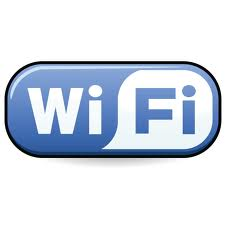
\includegraphics[width=5cm]{images/diplomarbeit/wifi_logo.jpeg}\\
            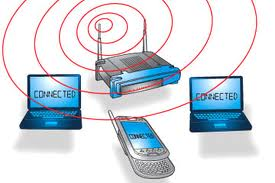
\includegraphics[width=5cm]{images/wifi.jpeg}\\
        \end{column}

        \begin{column}{7cm}
            \begin{itemize}
                \item Foor 
                \item Bar 
                \item Bal 
            \end{itemize}
        \end{column}
    \end{columns}
\end{frame}



\subsection{Bluetooth}
\begin{frame}
    \frametitle{Bluetooth}

    \begin{columns}[T]

        \begin{column}{5cm}
            
\includegraphics[width=5cm]{images/bluetooth_logo.jpeg}\\
            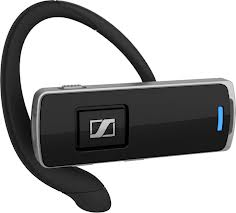
\includegraphics[width=5cm]{images/headset.jpeg}\\
        \end{column}

        \begin{column}{7cm}
            \begin{itemize}
                \item Foor 
                \item Bar 
                \item Bal 
            \end{itemize}
        \end{column}
    \end{columns}
\end{frame}

\subsection{ZigBee}
\begin{frame}
    \frametitle{ZigBee}

    \begin{columns}[T]

        \begin{column}{5cm}
            
\includegraphics[width=5cm]{images/zb_alliance_logo.gif}\\
            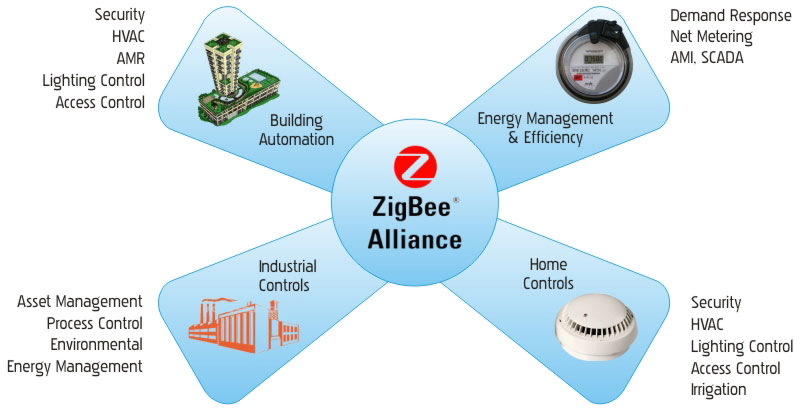
\includegraphics[width=5cm]{images/zigbee_development_big1.jpg}\\
            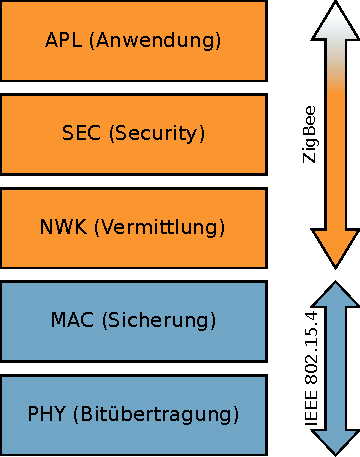
\includegraphics[width=5cm]{images/Zigbee_stack.pdf}\\
        \end{column}

        \begin{column}{7cm}
            \begin{itemize}
                \item Foor 
                \item Bar 
                \item Bal 
            \end{itemize}
        \end{column}
    \end{columns}
\end{frame}

\section{Markt�bersicht 2013}
\subsection{Verschiedene Module}
\begin{frame}
    \frametitle{ZigBee Module}
\end{frame}

\begin{frame}
    \frametitle{ZigBit}
\end{frame}

\begin{frame}
    \frametitle{XBee Pro}
\end{frame}

\begin{frame}
    \frametitle{freescale MC13202}
\end{frame}


\subsection{National Instruments}
\begin{frame}
    \frametitle{NI wireless sensor networks}

    \begin{columns}[T]

        \begin{column}{5cm}
            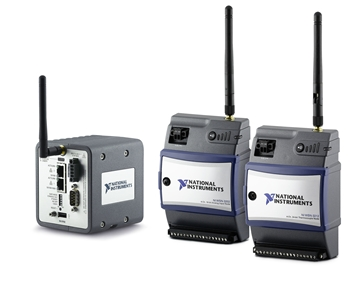
\includegraphics[width=5cm]{images/national instruments/RT_Gateway_and_Nodes_-_resized_JPEG.jpg}\\
        \end{column}

        \begin{column}{7cm}
            \begin{itemize}
                \item Foor 
                \item Bar 
                \item Bal 
            \end{itemize}
        \end{column}
    \end{columns}
\end{frame}

\subsection{Libelium}
\begin{frame}
    \frametitle{Libelium}

    \begin{columns}[T]

        \begin{column}{5cm}
            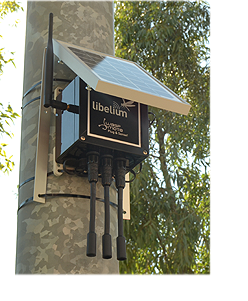
\includegraphics[width=5cm]{images/libelium/installation.png}\\
            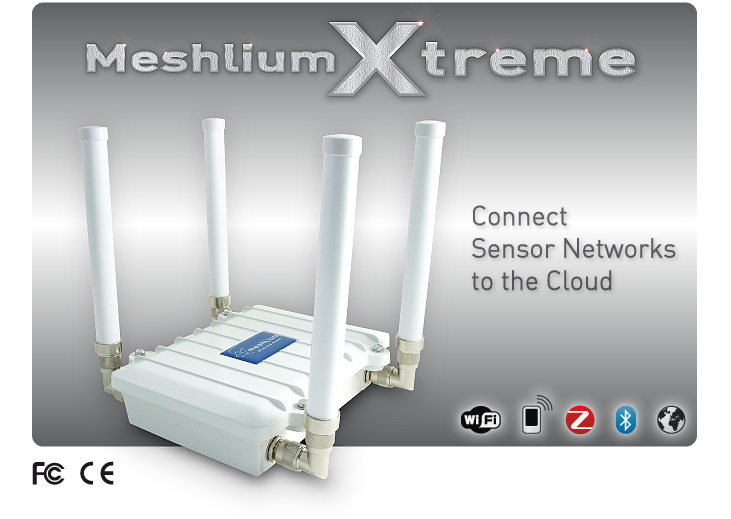
\includegraphics[width=5cm]{images/libelium/title_frontpage_description_eng.png}\\
        \end{column}

        \begin{column}{7cm}
            \begin{itemize}
                \item Foor 
                \item Bar 
                \item Bal 
            \end{itemize}
        \end{column}
    \end{columns}
\end{frame}
         

\subsection{Zum selber basteln}
\begin{frame}
    \frametitle{Zum selber basteln}
\end{frame}

\begin{frame}
    \frametitle{Arduino}
\end{frame}

\begin{frame}
    \frametitle{Rasperry Pi}
\end{frame}

\section{Security}
\subsection{ZigBee: WEP Reloaded}
\begin{frame}
    \frametitle{ZigBee: WEP Reloaded}
\end{frame}

\subsection{Kisbee}
\begin{frame}
    \frametitle{Kisbee}

    \begin{columns}[T]

        \begin{column}{5cm}
            \includegraphics[width=5cm]{images/netkismetwirelessandroidkisbee-1.1.jpeg}\\
            \includegraphics[width=5cm]{images/kissbee-select.png}\\
        \end{column}

        \begin{column}{7cm}
            \begin{itemize}
                \item Foor 
                \item Bar 
                \item Bal 
            \end{itemize}
        \end{column}
    \end{columns}
\end{frame}

\subsection{Ich sehe was, was Du nicht siehst: Introducing HackRF}
\begin{frame}
    \frametitle{HackRF}

    \begin{columns}[T]

        \begin{column}{5cm}
            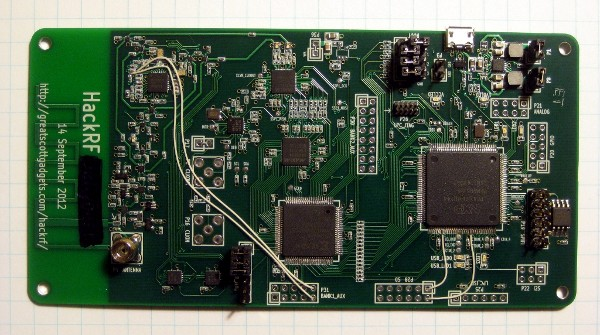
\includegraphics[width=5cm]{images/HackRF.jpg}\\
        \end{column}

        \begin{column}{7cm}
            \begin{itemize}
                \item Foor 
                \item Bar 
                \item Bal 
            \end{itemize}
        \end{column}
    \end{columns}

\end{frame}

\section{Aus der Alptraumabteilung}
\subsection{Smart dust}
\begin{frame}
    \frametitle{Smart dust}
\end{frame}

\subsection{Meine Kleidung funkt!}
\begin{frame}
    \frametitle{Meine Kleidung funkt!}
\end{frame}

\subsection{Fiat tenebrae: Geb�udeautomatisierung und smart metering}
\begin{frame}
    \frametitle{Geb�udeautomatisierung, Smart metering}
\end{frame}

\subsection{Dr Seltsam: Oder wie die Bombe lernte, mich zu lieben}
\begin{frame}
    \frametitle{Milit�rische Anwendungen}
\end{frame}
\end{document}
